\section{Methodology}
\label{sec:survey:methodology}

% General intro of what is happening in this chapter
% - Systematic approach to a survey (reproducible)
% - Section structure
The following section covers the methodology that is used throughout the systematic systems review. The idea of the systematic approach is to make the results as presented in this chapter reproducible. This is done by extensively detailing the methodology used and explaining the decisions we had to take. We present the guidelines, data sources and steps taken to reach the dataset used in the data synthesis. 

The remainder of this section is structured as follows. First, in \cref{sec:survey:methodology:strategy} we identify and discuss methods and techniques commonly used in systems surveys. Secondly, in \cref{sec:survey:methodology:approach}, we combine the methods and techniques identified, and present the strategy that we used to approach this survey. Subsequently, we introduce the research protocol that we established to conduct the survey.




\subsection{Defining a Strategy}
\label{sec:survey:methodology:strategy}

% Introduction to strategy definition


There are many methods and techniques out there to find, select or synthesize the data for a survey. The methodology and technique used throughout such a survey ultimately dictates the form a survey takes on and influences the results it produces. It is important to identify, compare and choose such methods and techniques that fit the needs of our system-focussed survey. 

In this section, we will present the identified methods that we can use for a survey. For each method, we discuss their advantages and disadvantages and whether we will use them in some form within the survey.

\subsubsection{Unguided Techniques}
\label{sec:survey:methodology:strategy:unguided}

% Analysis of common survey methods
% - Unguided Methods
% - Unguided Search -> Initial dataset
% - Backward Snowballing -> Enhange datase


\textit{Unguided search} is the first technique that we have identified. This technique is commonly used to produce an initial dataset of relevant literature on the topic. This process requires the researcher to traverse various digital libraries equipped with relevant keywords to produce the dataset. Another commonly used technique that we have identified is \textit{backward snowballing}. This is another unguided method often used as a complementary technique to expand the dataset and is achieved by searching for related papers in the reference section. By combining these techniques, a researcher can create a literature review based on the generated dataset. However, both of the techniques are unguided, and therefore the process is not reproducible. Using such unguided techniques can result in entirely different datasets if the process is to be repeated by another researcher, and thus does not produce much scientific value. 

% Analysis of common survey methods
% - Guided Methods
% - SLR (Kitchenham) -> Planning, Conducting, Reporting
% - Petersen -> comparative analysis guidelines
\subsubsection{Systematic Approach}
\label{sec:survey:methodology:strategy:systematic}

% SLR
To prevent any form of bias to have an effect on the process and results of a survey, we have to establish and utilize a systematic approach. We have identified a state-of-the-art methodology which aims to create a systematic process which will be used to guide this survey. The works of Kitchenham and Charters \cite{Kitchenham2007} introduce a battle-tested and auditable set of guidelines for literature reviews aimed at software engineering researchers  with the goal of promoting reproducibility. The introduced \textit{\gls{slr}} methodology consists of three steps, planning the review, conducting the review and reporting the review. We decided to use these guidelines as a baseline for the survey, as it aligns with our goals and environment.

In addition to the guidelines introduced by the \gls{slr} methodology, we utilize the guidelines as introduced in the works of Petersen et al. \cite{Petersen2008, Petersen2015}. The authors introduce a set of guidelines and techniques which can be used to conduct a mapping study on a given topic. Among the guidelines and techniques, the authors introduce a method to perform comparative analysis. These guidelines and methods align with our needs and goals to compare \gls{sm} systems in the field as stated by the formulated research question \ref{rq-1}. 

% MLR method (Garousi)
% - MLR (Garousi) -> Inclusion of GL
\subsubsection{Inclusion of Grey Literature}
\label{sec:survey:methodology:strategy:gl}

% - Previous lit survey -> Lack of PL
% - 2019 Secondary survey -> Lack of PL
% - Most content from the industry is GL
One of the drawbacks of the \gls{slr} method is that it only concerns \gls{pl}, which consists of published peer-reviewed academic articles. In our previous work, in which we have conducted a systematic literature review on the \gls{k8s} ecosystem, we came to the conclusion that this field lacked published and peer-reviewed articles. Additionally, previous secondary studies on the field came to the same conclusion \cite{service-mesh-survey}. The lack of published (formal) literature in the field makes it impossible for us to conduct the research to an extent which satisfies our goals. This led us to explore additional forms of literature. \Gls{gl} is a form of literature that does not belong in the formal category, and can be in the form of blog posts, videos or white papers. Exploratory research has shown that inclusion of \gls{gl} can be beneficial to our research, as most of the literature is presented in such form by the industry.

% - Introduction to MLR
To maintain a systematic approach with the inclusion of \gls{gl}, we had to define or find additional guidelines that supported this requirement. We have identified the state-of-the-art method for conducting a survey which enabled the inclusion of \gls{gl}. The \gls{mlr} methodology as introduced by Garousi et al. \cite{Garousi2019} adapts and extends the \gls{slr} method from Kitchenham et al. so that it can include both forms of literature. 

% MLR checklist table
\begin{table*}[t]
\centering
\resizebox{\linewidth}{!}{ %< auto-adjusts font size to fill line
    \begin{tabular}{@{}lll@{}}
    \toprule
    \# & Question & Answer \\
    \midrule
    1 & Is the subject “complex” and not solvable by considering only the formal literature? & Yes \\
    2 & Is there a lack of volume or quality of evidence, or a lack of consensus of outcome measurement in the formal literature? & Yes \\
    3 & Is the contextual information important to the subject under study? & Yes \\
    4 & Is it the goal to validate or corroborate scientific outcomes with practical experiences? & Yes \\ 
    5 & Is it the goal to challenge assumptions or falsify results from practice using academic research or vice versa? & No \\ 
    6 & Would a synthesis of insights and evidence from the industrial and academic community be useful to one or even both communities? & Yes \\ 
    7 & Is there a large volume of practitioner sources indicating high practitioner interest in a topic? & Yes \\ 
    \bottomrule
    \end{tabular}
} %< \resizebox
\caption[Questionnaire to decide whether to include \gls{gl}. ]{Questionnaire from the works of Garoussi et al. \cite{Garousi2019}, which helps to decide whether to include \gls{gl} in a literature survey.}
\label{tab:mlr-checklist}
\end{table*}

% - MLR requriements checklist
Additionally, the authors have created a checklist which can be used to verify the need for inclusion of \gls{gl} within a survey. If one or more of the questions in the checklist is answered with a \say{yes}, it indicates that \gls{gl} can be beneficial to the survey. We answered the questions in the provided checklist and the results of this can be seen in \cref{tab:mlr-checklist}. These results reaffirmed our requirement for \gls{gl} throughout the survey and made us adapt the guidelines as described by the methodology.




\subsection{Our Approach to a Systematic Survey}
\label{sec:survey:methodology:approach}
%  Summarize entire approach and present figure that shows this
% - SLR Leeading
% - MLR -> inclusiong of GL
% - Petersen -> comparitive analysis

In the previous section (\cref{sec:survey:methodology:strategy}), we identified several methodologies and guidelines which we can use to conduct a survey. We explained why we have chosen some of these guidelines for our systems survey and how they could apply to our research goals. The resulting strategy can be seen in more detail in the form of a flow chart in  \cref{fig:survey-methodology}. This figure depicts two of the three stages in from the \gls{slr} methodology, namely the planning phase and the conducting phase. It also lists all the deliverables of this systems survey (\designref{D1} - \designref{D5}). 

Up to this point, we have discussed two steps of the planning phase. This first step of the planning phase \designref{P1}, consists of establishing a need for the survey, which we did in \cref{sec:survey:introduction}. Next, we established our objectives \ref{obj:survey:1} - \ref{obj:survey:3} and research question \ref{rq-1} in \cref{sec:survey:objectives} which relates to process \designref{P2}.




% Support findings based on some perspectives
\begin{figure}[!t]
    \centering
    
    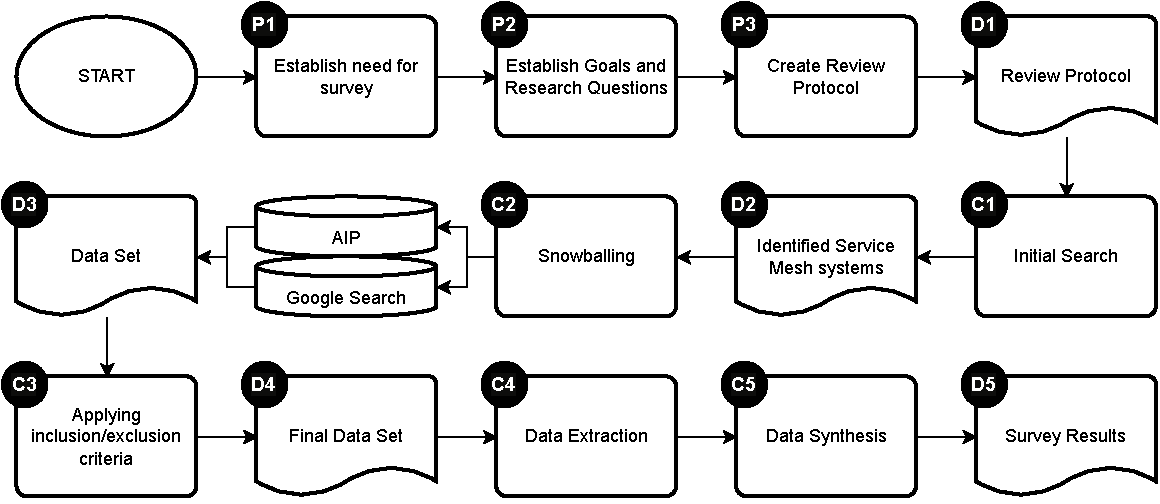
\includegraphics[width=\linewidth]{3_systems_survey/figures/survey-methodology}

    \caption[System survey approach.]{System survey approach.}
    \label{fig:survey-methodology}
\end{figure}




% % SLR Plannign phase
% % 1. Investigate need (rel. work)
% % 2. Objective of this research
% % 3. Formulate RQ.
% \subsection{Planning}
% \label{sec:survey:methodology:planning}

% \todo{Fix planning section}

% In line with the guidelines as proposed in the \gls{slr} methodology, we first conducted a planning stage. During this stage we have analysed relevant work and the need for a review as discussed in \cref{sec:survey:related-work}. After this, we formulated the goal and related research question of this survey as seen in \cref{sec:survey:goals}. The goal of this systems survey is to uncover the existing \gls{sm} systems in the landscape and provide an overview of characteristics that they have. By creating a data synthesis of the literature that we are able to find on this topic, we can produce a general framework to contain these systems. This is a stepping stone for the research that is conducted in the later chapters, in which we examine and evaluate the characteristics and performance properties of these systems in more detail. 



% SLR - Review Protocol
\subsection{Review Protocol}
\label{sec:survey:methodology:review-protocol}

% Review protocol consists of
% - Background, the rationale for the survey -> Goals
% - Research Questions that we intend to answer


% PL & GL
% - Search Strategy
% - Selection Criteria
% - Selection Procedures
% - Data Extraction



The review protocol is a fundamental aspect of the \gls{slr} methodology, it specifies the methods used to conduct the systems review in this thesis. A pre-defined protocol is required to reduce the possibility of any bias. Establishing the review protocol is part of our approach as specified in \cref{fig:survey-methodology} and depicts the process \designref{P3}.

In the remainder of this section, we introduce the components that establish the research protocol. In \cref{sec:survey:methodology:review-protocol:search-strategy}, we introduce the search strategy which is used to search for the relevant literature. In \cref{sec:survey:methodology:review-protocol:selection-criteria}, we establish the selection criteria which are used to filter the dataset which we obtained through the research strategy. Finally, in \cref{sec:survey:methodology:review-protocol:data-extraction}, we describe the methods used to extract and synthesize the data.



\subsubsection{Search Strategy}
\label{sec:survey:methodology:review-protocol:search-strategy}
% - Data Sources
% - Queries

To create a reproducible data set, we have to establish a search strategy which we use to obtain literature on the topic. The search strategy differs based on the type of literature, where different requirements apply for \gls{pl} and \gls{gl}.


% Data sources
% - AIP
% - Digital Libraries (DBLP, Aminer, Semantic Scholar)
% - Only established, well respected conferences
The first component that makes up the search strategy is related to the data sources. The Atlarge  team\footnote{\url{https://atlarge-research.com/}} has identified several digital libraries which are well established and which contain the leading publications in the field of distributed systems. Additionally, years of experience in the field led to the creation of a list of established and well-respected conferences. This consolidated knowledge led to the development of a software instrument \gls{aip}. This instrument is used to generate the initial dataset of \gls{pl} for this survey and query it. To establish a dataset of \gls{gl} in this survey, we use Google Search to identify relevant literature.

The second component of the search strategy is related to the search technique. Since the goal of this survey to compare state-of-the-art \gls{sm} systems, we first have to identify said systems. To achieve that, we first conducted exploratory research in the field. To reduce bias in this process, we first used the single identified secondary study \cite{service-mesh-survey} to obtain an initial set of \gls{sm} systems. After this, we identified the \gls{sm} systems that were part of official \gls{cncf} projects\footnote{\url{https://landscape.cncf.io/card-mode?category=service-mesh&grouping=category}}, as they have proven to be an authoritative entity in the field as discussed in \cref{sec:background:cncf}. This list was then complemented by results obtained from \gls{gl} using generic search queries. 


The final component of the search strategy is related to the search queries that we use to establish the resulting dataset. To find and identify the current state-of-the-art \gls{sm} systems, we used generic terms as described above. After this, we utilized a snowballing method in which we based the search queries on the identified systems. The final list of search queries used can be seen in \cref{tab:search-queries}. Queries \textbf{Q1} and \textbf{Q2} represent the queries used to obtain and expand the list of identified \gls{sm} systems, while \textbf{Q3} indicates the system-specific queries that were used. 

\begin{table}[t]
\centering
% \resizebox{\linewidth}{!}{ %< auto-adjusts font size to fill line
    \begin{tabularx}{\linewidth}{lXl}
    \toprule
    \# & Query & Search Strategy \\
    
    % Initial Search Queries
    \midrule
    \textbf{Q1} & Service Mesh & Initial Search \\
    \textbf{Q2} & Service Mesh Implementation & Initial Search \\

    % Queries Based on identified SM systems
    \midrule
    \textbf{Q3} & \textit{Identified Service Mesh Implementation} & Snowballing  \\
    
    \bottomrule
    \end{tabularx}
% } %< \resizebox
\caption{Search queries established in the review protocol.}
\label{tab:search-queries}
\end{table}

% \begin{table}[t]
% \centering
% % \resizebox{\linewidth}{!}{ %< auto-adjusts font size to fill line
%     \begin{tabular}{@{}lll@{}}
%     \toprule
%     \# & Query & Search Strategy \\
    
%     % Initial Search Queries
%     \midrule
%     \textbf{Q1} & Service Mesh & Initial Search \\
%     \textbf{Q2} & Service Mesh Implementation & Initial Search \\

%     % Queries Based on identified SM systems
%     \midrule
%     \textbf{Q3} & \textit{Identified Service Mesh Implementation} & Snowballing  \\
    
%     \bottomrule
%     \end{tabular}
% % } %< \resizebox
% \caption{Search queries established in the review protocol.}
% \label{tab:search-queries}
% \end{table}



\subsubsection{Selection Criteria}
\label{sec:survey:methodology:review-protocol:selection-criteria}
% Seperate Criteria for PL and GL
% Introduce the checklist and how it works
% display PL and GL checklist
Since we have decided to also include \gls{gl} in our survey, we decided to establish two sets of selection criteria since they are vastly different in terms of content and medium. For both types of literature, we establish a checklist. In this checklist, we define the guidelines that we use to either include or exclude a data point. Guidelines prefixed with a checkmark (\cmark) symbol indicate a reason to include a publication in the research, whereas the cross (\xmark) symbol indicates a reason for exclusion. 

The following checklist (\cref{list:checklist:pl}) contains a set of selection criteria that applies to the \gls{pl} that is obtained through the search process. For this, we apply a set of generic criteria in order to 

In addition to the search queries, we used a filter to filter out any results before 2014 since that the initial release date of \gls{k8s} \cite{kubernetes-launch}. This limits the results based on the scope of this research, which provides a focus on \gls{sm} systems in the \gls{k8s} ecosystem.

\begin{itemize}
    \item[(\cmark)] Publications that are written in English.
    \item[(\cmark)] Publications introducing novel concepts.
    \item[(\cmark)] Publications that focus on architectural problems and solutions.
    \item[(\cmark)] Publications performing performance analysis studies.
    
    \item[(\xmark)] Publications before 2014. 
    \item[(\xmark)] Publications that do not have \gls{sm} systems as the primary subject in the research. 
    \item[(\xmark)] Secondary or tertiary studies regarding \gls{sm} systems.
    \item[(\xmark)] Publications that are not full-text (e.g., small snippets or as part of a demo).
    
    \label{list:checklist:pl}
\end{itemize}


The following checklist (\cref{list:checklist:gl}) contains a set of selection criteria that applies to the \gls{gl} that is obtained through the search process. For this form of literature we had to establish a set of rigorous guidelines since it can otherwise result in numerous data entries or lead to a biased set of results. 

\begin{itemize}
    \item[(\cmark)] Publications that are written in English.
    \item[(\cmark)] Publications introducing novel concepts.
    \item[(\cmark)] Publications originating from well established and known organizations (e.g. \gls{cncf}, Google, Red Hat, etc.).
    \item[(\cmark)] Publications that supply official vendor or platform documentation.
    \item[(\cmark)] Publications in the form of blog posts from organizations or authorities in the field.
    \item[(\cmark)] Publications in the form of videos from talks or conferences related to the field.
    \item[(\cmark)] Source code repositories of open-source \gls{sm} systems (e.g., a GitHub repository).
    
    \item[(\xmark)] Publications in which we cannot validate the authority of an author (e.g., anonymous posts, or posts by someone not established in the field). 
    \item[(\xmark)] Publications which do not provide any novelty for the survey (e.g., tutorials on the technologies). 
    \item[(\xmark)] Publications that are not full-text (e.g., small snippets, parts of a demo or short social media excerpts such as tweets).
    
    \label{list:checklist:gl}
\end{itemize}


\subsubsection{Data Extraction}
\label{sec:survey:methodology:review-protocol:data-extraction}
% What kind of information is relevant to us
% Compare systems
% Observability
% Resilience
% Proxy Characteristics
% Protocol Support
% Security
% Meta


Once we have established a final dataset by filtering the dataset based on the selection criteria, we can start the data synthesis process. To achieve this, we first have to establish a set of data extraction guidelines. These guidelines have to be in line with the goals which of this survey. Since we want to compare  state-of-the-art \gls{sm} systems, we have to identify the key characteristics and properties  of such systems. Through the preliminary research conducted on the field, we understand the fundamentals of a \gls{sm} system and have identified the challenges it tries to solve. With this in mind, we try to identify and synthesize the data based on key areas.


% Observability
% Resilience
% Proxy Characteristics
% Protocol Support
% Security
% Meta
First off, we try to compare these systems based on their architectural approach. With this take, we can identify and compare \gls{sm} systems based on their design decisions, such as their control and data plane components. Secondly, we take a functional approach to synthesize these systems. By identifying sets of functionality, we can evaluate and compare these systems on domain-specific functionalities such as their observability, security, or resiliency characteristics. Furthermore, we take a meta analytical approach to these systems. With this, we try to establish certain aspects such as the number of users the system has, the development activity on the project, whether a project is open-source or not and the maturity of the system.